% Fig 4 wrapper: signed category and region deltas across states (headline figure).
% Real asset: fig4_deltas.pdf (rendered by fig4_deltas.py). Plan: PAPER_PLAN 6 / Fig 4.
\begin{figure}[!t]
\centering
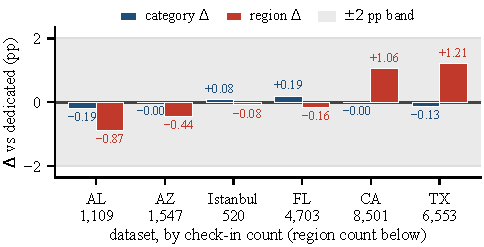
\includegraphics[width=0.79\columnwidth]{figs/fig4_deltas.pdf}
\caption{Signed differences between the joint model and the dedicated single-task models, ordered by
region count. The category differences (macro-F1) are small in both directions; on the region axis
(Acc@10), the two positive differences at the largest region vocabularies survive a Holm-corrected
superiority test, and all six lie inside the band, which is where non-inferiority is established.
The $\pm2$-point band is the margin registered for the region axis only.}
% [2026-09-06, camera-ready] Caption PORTED from the dissertation chapter (author decision B-27,
% 2026-09-02; articles/dissertacao/src/chapters/5_mobiwac/06_results.tex, figure environment),
% replacing the src_fix caption that still read "stays within a fifth of a point everywhere"
% (plan item D2 of the port audit). The interim rewrite of earlier today is superseded by the
% approved text. Values: CAMERA_READY section 3.1/3.2.
\label{fig:deltas}
\end{figure}
